In this section we will provide and overview of the relevant background and context for this thesis. First introducing the software engineering lifecycle and the rising role of GenAi/LLMs in it. The Second part showcases the evolution and state of APR and explores existing approaches.

\section{Software Engineering}
In the follwing section introduces the software engineering lifecycle, the role of code hosting platforms, and the importance of Continuous Integration and Continuous Deployment (CI/CD) in modern software development.
\subsection{Software Development Lifecycle}
Engineering Software is complex and including multiple stages. For structuring this work diffrent Software Developemnt Lifecycle Models have been introduced. Software Development Lifecycle Models evolve constantly to adapt to the chanign needs of creating software. The most promising and widely used model is the Agile Software Development Lifecycle \cite{rupareliaSoftwareDevelopmentLifecycle2010}.

The Agile lifecycle brings an interative approach to development, focusing on collaboration, feedback and adaptivity. The Goal frequent delivery of small functional features of software, allowing for continuous improvement and adaptation to changing requirements. Agile can be used with multiple frameworks like Scrum or Kanban but follows a similar approach. \cite{rupareliaSoftwareDevelopmentLifecycle2010}.

\begin{figure}[htbp]
    \centering
    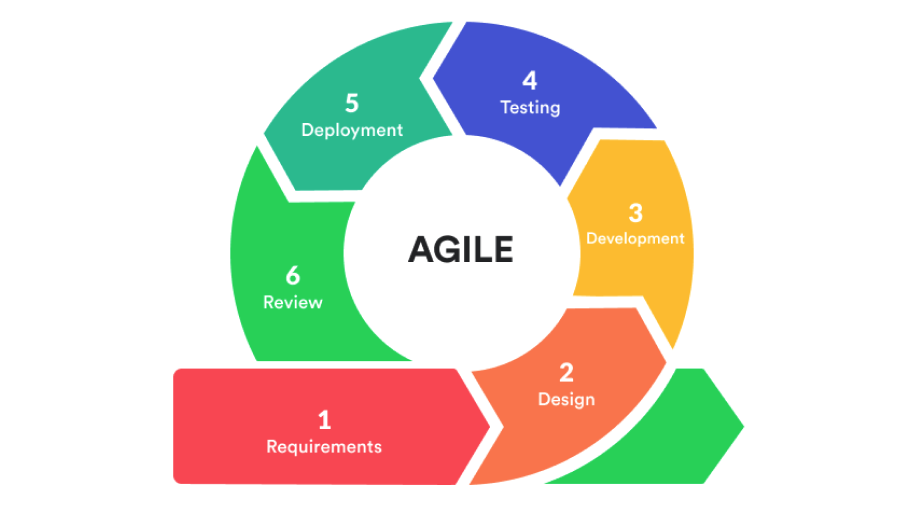
\includegraphics[width=0.8\textwidth]{images/agile-cycle.png}
    \caption{Agile Software Development Lifecycle}
    \label{fig:agile-cycle}
\end{figure}

A Agile Software Development Lifecycle iteration consists of several key stages like in Figure starting with planning phase where requirements for the iterartion are gathered and pritorized.

Since agile focuses adaptivity arising bugs can alter iterations if priotirised and therefore slow down delivery of features. APR is supposed to help with this problem by accelerating the process of fixing bugs.

Software development is moving towards lightly coupled microsversives which results in more repositories which are smaller in scale tailored towards a specialzed domain. This trend is driven by the need for flexibility, scalability, and faster development cycles. Smaller code repositories allow teams to work on specific components or services independently, reducing dependencies and enabling quicker iterations. This approach aligns with modern software development practices, such as microservices architecture and agile methodologies.
With this trend developers work on multiple projects at the same time, which can lead to more interrupptions and context swtiching when problems arise and priorities shift.



\subsection{Continuous Integration}

For accelerating the delviery of software in an iteration continous integration has become a standard in agile software development. 
Continuous Integration (CI) allows for frequenct code integration into a code repository. Ci often integrates automated building and testing giving rapid feedback right where the changes are made on the hosted repository.


Problems can be long build durations and high maintance \cite{ugwuezeContinuousIntegrationDeployment2024}

CI supports aspects like fast delivery, fast feedback, enhanced collaboration which are ciritcal for agile software development. 

\subsection{project hosting platforms}
Most software projects are hosted on platform like Github. But github is more than just a storage for repositories. It provides tools and feature for the complete software development lifecycle. Project hosting, verssion control, bug and issue tracking, project management, backups, collaboration, and documentation. \cite{abrahamssonAgileSoftwareDevelopment2017}




github is whre open soruces lives and development takes place. It is a platform that allows developers to host, share, and collaborate on code repositories. GitHub provides version control, issue tracking, and collaboration tools, making it a popular choice for open-source projects and software development teams.

allows for integration of systems like rennovate


\section{LLMs in Software Engineering}

modern large language models have billions of paramters, are pre-tained on massive codesbases which results in extraordinary capbilites in this area  \cite{chenUnveilingPitfallsUnderstanding2025}.

% TODO cite 
problems with llms are: Information leakage, hallucinations, and security issues

first LLms now research is looking into developing and improving workflows leveraging LLMs \cite{puvvadiCodingAgentsComprehensive2025}.

% TODO cite 
problems wi
looking into Agents using tools, LLMs + RAG,

\section{Automated Programm Repair}

Automated Program Repair (APR) helps developers fix bugs

localization, repair, and validation


\subsection{Evolution of Automated Program Repair}
% TODO cite 
Earliest APR techniques were based on version control history, using the history to roll back to a previous version of the code part, where no issues were present. This approach, while effective in some cases, often lacked the ability to perserve new features. (more like instant rollback)
history based

--- search based repair,

---semantic based repair,

---tempalte based repair,
apply predefined transformtions to the code based on rules

---The emerge of llm based techniques
LLM based APR techniques have demonstrated siognificant uimrpovemetns over all other state of the art technqiues, benfitintting from theor coding knowledge \cite{hossainDeepDiveLarge2024}

Agent Based
agent based system improve fixing abilites by probiding llms the ability to interact with the code base and the environment, allowing them to plan their actions  \cite{yangSWEagentAgentComputerInterfaces2024}.

llms lay the groundwork of a new APR paradigm \cite{chenUnveilingPitfallsUnderstanding2025}

complex agent arcitectures produce good results espically paired with containerized environments. Emphasis on quality insureance and Devops practices \cite{puvvadiCodingAgentsComprehensive2025}


modern aprs usally consist of multiple stages, including localization, repair, and validation. These stages are often implemented as separate modules, allowing for flexibility and modularity in the repair process \cite{yangSWEagentAgentComputerInterfaces2024}.

\subsection{Related Work - Existing Systems}


end to end without llms Sapfix from Facebook. Fixing bugs in production envrioments lowerring incidents mean time of recovery significantly \cite{margineanSapFixAutomatedEndtoEnd2019}

FixAgent \cite{leeUnifiedDebuggingApproach2024}

swe agent \cite{yangSWEagentAgentComputerInterfaces2024}

Agentless minimal system \cite{xiaAgentlessDemystifyingLLMbased2024}
claims exsiting systems are too complex and compute/costs intensive.
lacks the ability to control the decision planning.
they use a minimalist approach using localization, repair and validation.


this appraoch inspried the thesis to test how a simple approach will perform in a real world scendario on a code hosting platform.


--point out areas where current systems see limitation

-- during the research for this thesis, full integrations where published by companies like OpenAI Codex and Github Copilot - but these are not open source


\subsection{APR in CI Context}

CI allows seemless integration...
this way there is no harmfull code executed on own machiene, its encapsulated mutliple times container in Ci runner
